\scanpage{335}
\mspage{5}

\uline{Question} Y-a-t-il d'autres objets \deleted{\unsure{tot.}} $W_\infty$-\unsure{asphérique|asphériques} de $\mathrm{Cat}$, que les catégories ayant un objet final ? Je suspecte à présent que non - donc que l'on ne peut améliorer \deleted{\unsure{substanti}} \unsure{ellement|tellement} sur la notion déjà connue d'immersion ouverte de Dwyer.

\figure{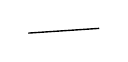
\begin{tikzpicture}\draw[line width=.5pt] (0,0) -- (.9,.06);\end{tikzpicture}}

Dans le diagramme

\diagram{$(\alpha)$\qquad\begin{tikzcd}[ampersand replacement=\&,column sep=large]
 U\arrow[r,hook,"i"]\arrow[d,dash,"p"'] \& X\arrow[d,dash,"q"] \& T\arrow[l,dashed,hook',"j"']\arrow[d,"\mathrm{iso}"]\\
 U'\arrow[r,hook,"i'"']\arrow[ur,phantom,"\text{\scriptsize cocart. et cart.}" description] \& X'\& T'\arrow[l,dashed,hook',"j'"]
\end{tikzcd}}

prenons $U=\Psi$, $T=\{t\}=e$ catégorie finale, $t$ objet final \deleted{de $X$} i.e. \deleted{$\unsure{E|H|\square}$}

\[
 H_t=\bigl(u\longmapsto\operatorname{Hom}_X(u,t)\bigr)=e_{\unsure{U|u}}\in\mathrm{Ob}\,U^\wedge
\]

% slanted
\margin{i.e. $X$ déduit de $U=\Psi$ en lui rajoutant un objet final $t$ donc $X\simeq\Delta^1\times\Delta^1$}

% slanted
\margin{\diagram{\begin{tikzcd}[ampersand replacement=\&,column sep=small,row sep=small,execute at end picture={\draw[rounded corners=5pt] ([xshift=-5pt,yshift=6pt]TL.north west) -- ([xshift=8pt,yshift=6pt]TL.north east) -- ([xshift=8pt,yshift=-8pt]TL.south east) -- ([xshift=6pt,yshift=8pt]BR.north east) -- ([xshift=7pt,yshift=-5pt]BR.south east) -- ([xshift=-7pt,yshift=-6pt]BL.south west) -- cycle;}]
 |[alias=TL]|\phantom{x}\arrow[r] \& \phantom{x}\\
 |[alias=BL]|\cdot\arrow[u]\arrow[r] \& |[alias=BR]|\phantom{x}\arrow[u]\\
 \Psi\arrow[u,shorten >=4pt] \&
\end{tikzcd}}}

Prenons pour $U'$ la cat. dont il est question dans la ``prop.'' hypothétique (et \unsure{fausse}) p 1, \inserted{avec $b=c$,} plus précisément une catégorie \deleted{\unsure{ab}} avec deux objets $b$ et $b\times b$, un groupe \inserted{(voire un monoïde)} $G$ d'endom. de $b$, et les autres flèches celles qui s'en \unsure{déduisent}, en exigeant que $b\times b$ soit bel et bien le carré cartésien de $b$. On trouve une catégorie cofibrée (\deleted{\unsure{non}} propre) sur la cat. $T$ opposée de celle des ens finis de la forme $\{0\}$ et $\{0,1\}$ (deux objets) avec comme fibres $B_G$ et $B_{G\times G}$ respectivement.

($B_{\unsure{\Pi|\pi|R}}:=$ cat. avec un seul objet, et monoïde d'endomorphismes $\unsure{R|\Pi|\pi}$.) Le foncteur \unsure{2|?}

\[
 U=\Psi\longrightarrow U'
\]

est celui donné par le diagramme

% archive sheet number: 335
